\documentclass[slovak]{article}
\usepackage[dvips]{graphicx}        % to include images
\usepackage{pslatex}	    % to use PostScript fonts
\usepackage[T1]{fontenc}
\usepackage[utf8]{inputenc}
\usepackage{pslatex}

\usepackage{tabularx} % tabulky na celu sirku strany
\usepackage{graphicx} %graphics files inclusion
\usepackage{longtable}
\usepackage{multirow}
\usepackage{mathtools}
\usepackage{listings}
\usepackage{pdfpages}
\usepackage{amsmath}
\usepackage{lscape}

\hyphenation{re-fe-ren-čné}
\hyphenation{de-kom-po-zí-cie}
\hyphenation{ma-xi-mál-ny}
\hyphenation{ma-xi-mál-na}
\hyphenation{al-go-rit-mus}
\hyphenation{e-xakt-né-mu}

\begin{document}

\title{Problém batohu - 2. úloha \\[5mm] MI-PAA, zimný semester 2014}
\author{Martin Klepáč}
\date{\today}

\maketitle

\section{Definícia problému}

Problém batohu (knapsack problem) je jeden z NP-ťažkých problémov. Pokiaľ máme k dispozícii množinu predmetov, pričom každý predmet má svoju váhu, cenu, a maximálnu nosnosť batohu, potom je naším cieľom vybrať predmety do batohu tak, aby sme maximalizovali ich cenu a pritom celková hmotnosť predmetov nepresiahla maximálnu povolenú nosnosť batohu.

\section{Formát vstupu}

Formálne, vstup vyjadríme pomocou

\begin{itemize}

\item \emph{n} = počet predmetov

\item \emph{M} = maximálna nosnosť batohu

\item \emph{vektor v} = hmotnosť jednotlivých predmetov

\item \emph{vektor c} = hodnota (cena) jednotlivých predmetov

\end{itemize}

Výstupom algoritmu je vektor \emph{x}, ktorý udáva prítomnosť/neprítomnosť daného predmetu vo výbere. Ďalej požadujeme informáciu o celkovej hmotnosti predmetov v batohu a ich súhrnú hodnotu pre najlepší výber.


\section{Rozbor možných variant}

V prvej úlohe sme problém batohu riešili hrubou silou, ktorá nám poskytla referenčné riešenie na úkor exponenciálnej zložitosti. Pre dosiahnutie približného výsledku sme ďalej realizovali heuristiku cena-váha, podľa ktorej sme pridávali elementy do batohu s najvyšším pomerom cena-váha, až kým nedošlo k presiahnutiu maximálnej nosnosti batohu.

V druhej úlohe budeme riešiť problém batohu trojicou algoritmov. Konkrétne sa jedná o riešenie s použitím orezávania stavového priestoru (označované ako branch-and-bound), algoritmus dynamického programovania a v neposlednom rade algoritmus FPTAS. Zatiaľ čo prvé dve riešenia poskytujú exaktné výsledky, FPTAS podobne ako heuristika cena-váha predstavuje aproximatívne riešenie.

Riešenie označované ako branch-and-bound je založené na myšlienke orezávania stavového priestoru. Pokiaľ máme k dispozicii určitý subvýber skladajúci sa z \emph{p} elementov za podmienky \emph{p<n}, potom za určitých okolností nemusíme riešiť všetky možné výbery, ktoré by z tohto subvýberu mohli vzniknúť. Jednou z týchto okolností môže byť fakt, že váha súčasných \emph{p} elementov prekračuje maximálnu nosnosť batohu, a teda akékoľvek riešenie pozostávajúce z takéhoto subvýberu je neplatné - orezávanie priestoru zvrchu. Častejšou variantou je orezávanie priestoru zo spodu, kde platí, že v prípade pridania všetkých zostávajúcich prvkov do existujúceho subvýberu, výsledná cena výberu bude nižšia ako existujúce maximum.

Riešenie problému batohu metódou dynamického programovia je svojím spôsobom podobné rekurzívnemu riešeniu, ktoré som aplikoval v prvej úlohe, brute force algoritmus. Rekurzia a dynamické programovanie majú spoločný základ v rozklade problému na podproblémy. V čom sa zásadne líšia, je fakt, že rekurzíva subproblémy počíta opakovane, zatiaľ čo dynamické programovanie subproblém vypočíta raz a jeho výsledok si uloží do pamäťových štruktúr. Dynamické programovanie realizujeme pomocou dekompozície podľa kapacity.

Aproximatívne riešenie predstavuje algoritmus FPTAS, fully polynomial-time approximation scheme. FPTAS k svojmu behu využíva koncept dynamického programovania, riešenie subproblémov ukladá do pamäte. Jeho aproximácia spočíva v zanedbaní least significant bitov cien jednotlivých predmetov - tentokrát bolo potrebné realizovať algoritmus dynamického programovania dekompozíciou podľa ceny. Na rozdiel od heuristiky cena-váha, ktorá riešenie aproximuje, je možné FPTAS algoritmus parametrizovať, a tým de facto určovať mieru nepresnosti.

\section{Rámcový popis postupu}

Začneme implementáciou riešenia branch-and-bound, následne postúpime k algoritmu dynamického programovania s dekompozíciou podľa kapacity batohu. Overíme, že obe riešenia poskytujú exaktné výsledky porovnaním s referenčným brute force algoritmom. Ďalej, implementujeme algoritmus FPTAS, ktorý interne využíva dynamické programovanie s použitím dekompozície podľa ceny. Pri tomto riešení budeme merať mieru nepresnosti v závislosti od parametru počtu bitov - \emph{i}, ktoré budeme zanedbávať v cene jednotlivých predmetov. V závere výsledky jednotlivých riešení zobrazíme ako v textovej podobe (tabuľka), tak vo forme príslušných grafov.


\section{Popis kostry algoritmu}

Algoritmus branch-and-bound je založený na prehľadávaní stavového priestoru, ktoré je realizované formou algoritmu BFS (breadth first search) s ukladaním prvkov do fronty. Potom každý prvok fronty predstavuje určitý subvýber, kde prvých \emph{i} elementov (\emph{i<n}) je daných, t.j. buď sa vo výbere nachádzajú alebo nenachádzajú, a o osude zvyšných \emph{(n-i)} elementov nie je zatiaľ rozhodnuté. Ľavý potomok elementu vyjadruje obsiahnutie ďalšieho prvku v subvýbere, zatiaľ čo pravý potomok elementu neobsahuje ďalší prvok v subvýbere. Vo výsledku tak budujeme binárny strom, ktorého hĺbka odpovedá počtu prvkov na vstupe. Pre každý uzol počítame jeho maximálny potenciálny profit - k váhe a cene existujúceho subvýberu pripočítavame ďalšie prvky na základe najvyššieho pomeru cena-váha, až kým nedôjde k pretrhnutiu batohu. Pokiaľ je maximálny potenciálny profit uzla menší ako aktuálne najvyššia dosiahnutá cena výberu, takýto subvýber označíme za neperspektívny (orezávanie zo spodu). Prerekvizitou tohto algoritmu je teda usporiadanie elementov podľa najlepšieho pomeru cena-váha zostupne.

Druhé riešenie predstavuje algoritmus dynamického programovania s použitím dekompozície podľa kapacity. V ňom riešenie problému skladáme z už vyriešených subproblémov, ktorých výsledky uchovávame v 2D poli o veľkosti [\emph{počet prvkov + 1}] x [\emph{maximálna nosnosť batohu +1}]. Toto pole nám fakticky odpovedá na nasledujúcu otázku - pokiaľ máme k dispozícii prvých \emph{i} prvkov (\emph{i<=n}) a postupne sa zväčšujúcu kapacitu \emph{c} až do (\emph{c<=nosnosť batohu}), aká je maximálna dosiahnuteľná cena výberu? Výsledok teda nájdeme po vyplnení celého poľa na pozícii [\emph{počet prvkov}][\emph{nosnosť batohu}].

Algoritmus FPTAS predstavuje posledné implementované riešenie problému batohu. Interne využíva algoritmus dynamického programovania s dekompozíciou podľa ceny, ktorý rieši inverzný problém batohu. K jeho implementácii potrebujeme 2D pole o veľkosti [\emph{počet prvkov + 1}][\emph{súčet cien prvkov na vstupe + 1}]. Potom sa pri riešení inverzného problému batohu snažíme minimalizovať výslednú váhu výberu, pokiaľ máme zadanú celkovú cenu výberu. Využitie algoritmu FPTAS spočíva v tom, že umelo znižuje ceny všetkých predmetov na vstupe (implementačne riešené posunom o \emph{i} bitov doprava, t.j. delením ceny hodnotou $2^i$), čím dochádza k zmenšeniu hore popísanej tabuľky. Po vyplnení tabuľky hľadáme s použitím všetkých prvkov prvú hmotnosť, ktorá je nižšia ako maximálna nosnosť batohu - príslušná cena potom predstavuje maximálnu cenu výberu s dodržaním pravidla o nosnosti batohu. Túto cenu potom spätne posunieme o \emph{i} bitov doľava, čo odpovedá vynásobeniu hodnotou $2^i$.

\section{Výsledky}

Opäť máme k dispozícii 64-bitový Linuxový host, na ktorom spúšťame kód napísaný v jazyku C++ pre všetky inštancie až do \emph{n=40}. Problém nastáva pri vyšších inštanciách v súvislosti s algoritmom branch-and-bound, pretože pre každé \emph{n} existuje inštancia, ktorá núti program prehľadať celý stavový priestor (nevzniká možnosť orezania neperspektívnych vetiev). Takéto prípady sa ukázali byť na testovanom stroji v rozumnom čase neriešiteľné z dôvodu toho, že program musí do fronty uložiť prakticky všetky možné subvýbery, čo bohužiaľ neumožňuje limitované množstvo pamäte (4 GB). Po zaplnení main memory preto dochádza k swapovaniu, ktoré výrazne zhoršuje výsledky aj v porovnaní s brute force algoritmom, ktorý sa celý pri porovnateľnej veľkosti inštancie zmestil do pamäte. Z tohto dôvodu bol voči daným vzorkám vytvorený špeciálny test, ktorý sa spustí pred samotným branch-and-bound algoritmom a ktorý nastaví dosiaľ najlepšie riešenie na cenu predmetu, ktorý sám zaberá celú kapacitu batohu.

Výsledky sú uvedené v trojici tabuliek. Tabuľka \ref{tab1} zobrazuje absolútne časy trvania jednotlivých implementácií v závislosti od počtu prvkov na vstupe. Jedná sa o priemerné hodnoty spomedzi 50 inštancií pre každé \emph{n}. V tabuľke pre porovnanie uvádzam trvanie brute-force algoritmu do veľkosti inštancie \emph{n=30}. Tabuľky \ref{tab2} a \ref{tab3} zobrazujú priemernú relatívnu chybu resp. maximálnu chybu spomedzi 50 inštancií dosiahnutú algoritmom FPTAS(i) pre \emph{i=1..4}.

Grafické vyjadrenie rovnakých dát prikladám ako obrázky \ref{gr:graf1} až \ref{gr:graf3}. Graf \ref{gr:graf1} zobrazuje priemerné trvanie behu jednotlivých implementácií z druhej úlohy, t.j. branch-and-bound, dynamické programovanie a FPTAS algoritmus s paremetrami \emph{i=0} až \emph{i=6} (do tabuľky \ref{tab1} sa mi nepodarilo z priestorových dôvodov zaniesť časy pre FPTAS(5) a FPTAS(6)). Na zobrazenie hodnôt na Y-osi som použil logaritmické merítko, pretože kým trvanie behu algoritmu branch-and-bound rastie s narastajúcou veľkosťou vzorky exponenciálne, ostatné funkcie rastú rádovo pomalšie. Graf \ref{gr:graf2} zobrazuje priemernú relatívnu chybu ceny výsledného výberu pri použití algoritmu FPTAS s parametrom \emph{i=1..6}. FPTAS s parametrom \emph{i=0} reprezentuje algoritmus dynamického programovania s použitím dekompozície podľa ceny, a teda poskytuje exaktné výsledky. Konečne, graf \ref{gr:graf3} zobrazuje maximálnu relatívnu chybu spomedzi 50 inštancií pre FPTAS(i) v rozmedzí \emph{i=0} až \emph{i=6}. Opäť, grafy \ref{gr:graf2} a \ref{gr:graf3} naviac obsahujú merania pre hodnoty FPTAS(5) a FPTAS(6).

\begin{landscape}
\begingroup
\scriptsize

\begin{table}\centering
	\begin{tabularx}{\linewidth}{ | X | X | X | X | X | X | X | X | X |}
	  \hline                       
					& 	\textbf{BF}	& \textbf{BB}	& \textbf{DP}		& \textbf{FPTAS(0)} 	& \textbf{FPTAS(1)}	& \textbf{FPTAS(2)}		& \textbf{FPTAS(3)}			& \textbf{FPTAS(4)}\\ \hline
	  \textbf{n=4} 	& $6.79.10^{-7}$			& 0.000 003 	& 0.000 006	 		& 0.000 025			& 0.000 017			& 	0.000 013			& 0.000 007		&	0.000 003 	\\ \hline
	  \textbf{n=10} & 0.000 270					& 0.000 042 	& 0.000 022 		& 0.000 273			& 0.000 160			& 	0.000 079			& 0.000 045 	&	0.000 018   \\ \hline
	  \textbf{n=15} & 0.004 196					& 0.000 273 	& 0.000 057 		& 0.000 547			& 0.000 242			& 	0.000 196			& 0.000 101 	&	0.000 046	\\ \hline
	  \textbf{n=20} & 0.140 290					& 0.001 459 	& 0.000 082 		& 0.000 842			& 0.000 421			& 	0.000 334			& 0.000 112 	&	0.000 078	\\ \hline
	  \textbf{n=22} & 0.580 960					& 0.002 496 	& 0.000 096 		& 0.001 066 		& 0.000 701			& 	0.000 264 			& 0.000 151 	&	0.000 093	\\ \hline
	  \textbf{n=25} & 4.828						& 0.009 033 	& 0.000 125 		& 0.001 371 		& 0.000 901			& 	0.000 506			& 0.000 168 	&	0.000 128	\\ \hline
	  \textbf{n=27} & 19.584					& 0.025 800		& 0.000 184 	 	& 0.001 723 		& 0.001 122			& 	0.000 384			& 0.000 192 	&	0.000 144	\\ \hline
	  \textbf{n=30} & 167.61					& 0.077 862		& 0.000 205		 	& 0.002 018			& 0.001 029			& 	0.000 490			& 0.000 246 	&	0.000 182	\\ \hline
	  \textbf{n=32} & N/A						& 0.151 140		& 0.000 247		 	& 0.002 277			& 0.001 251			& 	0.000 791			& 0.000 261 	&	0.000 126	\\ \hline
	  \textbf{n=35} & N/A						& 0.181 685		& 0.000 308		 	& 0.002 694			& 0.001 328			& 	0.000 900			& 0.000 319 	&	0.000 157	\\ \hline
	  \textbf{n=37} & N/A						& 0.292 665		& 0.000 368		 	& 0.003 047			& 0.001 429			& 	0.000 843			& 0.000 339 	&	0.000 245	\\ \hline
	  \textbf{n=40} & N/A						& 0.484 644		& 0.000 421 	 	& 0.003 556			& 0.001 709			& 	0.000 822			& 0.000 412 	&	0.000 210	\\ \hline
	\end{tabularx}
\caption{Priemerné trvanie behu v sekundách pre varianty brute-force (BF), branch-and-bound (BB), dynamického programovania (DP) s dekompozíciou podľa kapacity a FPTAS algoritmu s daným paremetrom \emph{i}}
\label{tab1}
\end{table}
\endgroup
\end{landscape}

\begin{table}\centering
	\begin{tabularx}{\textwidth}{ | X | X | X | X | X |}
	  \hline                       
					& \textbf{FPTAS(1)} 	& \textbf{FPTAS(2)} & \textbf{FPTAS(3)} 	& \textbf{FPTAS(4)}\\ \hline
	  \textbf{n=4} 	& 0.41 					& 1.05 				&  2.43 				& 5.09	\\ \hline
	  \textbf{n=10} & 0.33 					& 1.04 				&  2.44 				& 5.06	\\ \hline
	  \textbf{n=15} & 0.37 					& 1.16 				&  2.83 				& 5.75	\\ \hline
	  \textbf{n=20} & 0.34 					& 1.02 				&  2.41 				& 5.40	\\ \hline
	  \textbf{n=22} & 0.34 					& 1.05 				&  2.41 				& 5.09	\\ \hline
	  \textbf{n=25} & 0.32 					& 0.99 				&  2.27 				& 5.04	\\ \hline
	  \textbf{n=27} & 0.36 					& 1.03 				&  2.43 				& 5.14	\\ \hline
	  \textbf{n=30} & 0.32 					& 0.98 				&  2.29 				& 5.04	\\ \hline
	  \textbf{n=32} & 0.32 					& 0.96 				&  2.28 				& 4.94	\\ \hline
	  \textbf{n=35} & 0.32 					& 0.96 				&  2.24 				& 4.93	\\ \hline
	  \textbf{n=37} & 0.32 					& 0.99 				&  2.28 				& 4.95	\\ \hline
	  \textbf{n=40} & 0.32 					& 0.99 				&  2.27 				& 4.89	\\ \hline
	\end{tabularx}
\caption{Priemerná relatívna odchýlka ceny výsledného výberu realizovaného FPTAS algoritmom v percentách}
\label{tab2}
\end{table}

\begin{table}\centering
	\begin{tabularx}{\textwidth}{ | X | X | X | X | X | }
	  \hline                       
				& \textbf{FPTAS(1)} 	& \textbf{FPTAS(2)} & \textbf{FPTAS(3)} & \textbf{FPTAS(4)}\\ \hline
	  \textbf{n=4} 	& 2 	& 4 	&  12 		&	20 	\\ \hline
	  \textbf{n=10} & 1.01 	& 3.03 	&  4.32 	&	9.18\\ \hline
	  \textbf{n=15} & 0.67 	& 1.76 	&  4.50 	&	8.66\\ \hline
	  \textbf{n=20} & 0.55 	& 1.50 	&  3.50 	&	7.51\\ \hline
	  \textbf{n=22} & 0.57 	& 1.58 	&  3.64 	&	8.35\\ \hline
	  \textbf{n=25} & 0.57 	& 1.42 	&  3.19 	&	6.89\\ \hline
	  \textbf{n=27} & 0.59 	& 1.47 	&  3.35 	&	7.77\\ \hline
	  \textbf{n=30} & 0.47 	& 1.47 	&  3.03 	&	7.26\\ \hline
	  \textbf{n=32} & 0.58 	& 1.48 	&  3.26 	&	7.11\\ \hline
	  \textbf{n=35} & 0.43 	& 1.38 	&  3.29 	&	7.08\\ \hline
	  \textbf{n=37} & 0.54 	& 1.68 	&  3.45 	&	6.61\\ \hline
	  \textbf{n=40} & 0.45 	& 1.43 	&  3.20 	&	6.10\\ \hline
	\end{tabularx}
\caption{Maximálna odchýlka ceny výsledného výberu realizovaného FPTAS algoritmom v percentách}
\label{tab3}
\end{table}


\section{Diskusia}

V druhej úlohe sme implementovali trojicu algoritmov. Zložitosť algoritmu branch-and-bound je exponenciálna a v najhoršom prípade môže viesť k prehľadaniu kompletného stavového priestoru. Vo väčšine prípadov však orezávanie zdola pomocou ceny (a v menšej miere zhora pomocou kapacity) vedie k výraznému zrýchleniu v porovnaní s pôvodným brute force algoritmom. Algoritmus dynamického programovania je založený na postupnom vyplňovaní tabuľky, pomocou ktorej riešenie problému skladáme z riešení subproblémov. Veľkosť tejto tabuľky sa líši v závislosti od použitého typu dekompozície. V mojom prípade som implementoval oba spôsoby, pod označením "dynamické programovanie" som využil dekompozíciu podľa kapacity, v algoritme FPTAS som využil dekompozíciu podľa ceny. Zložitosť algoritmu dynamického programovania je pseudo-polynomiálna, čím vyjadrujeme, že nezávisí výhradne nad počtom vstupných dát. Dynamické programovanie poskytuje presné výsledky. Naproti tomu algoritmus FPTAS neposkytuje exaktné výsledky, ale na druhej strane je realizovateľný v polynomiálnom čase a naviac je parametrizovateľný, t.j. mieru chyby si môžeme meniť. Napríklad, pri zanedbaní posledných 4 bitov cien predmetov došlo k relatívnej chybe približne 10 percent.

\section{Literatúra}

\begin{itemize}
	\item Foundations of Algorithms Using C++ Pseudocode, Richard E. Neapolitan, Kumarss Naimipour
	\item http://www.programming-techniques.com/2013/07/solving-knapsack-problem-using-dynamic.html
\end{itemize}


\begin{figure}\centering
	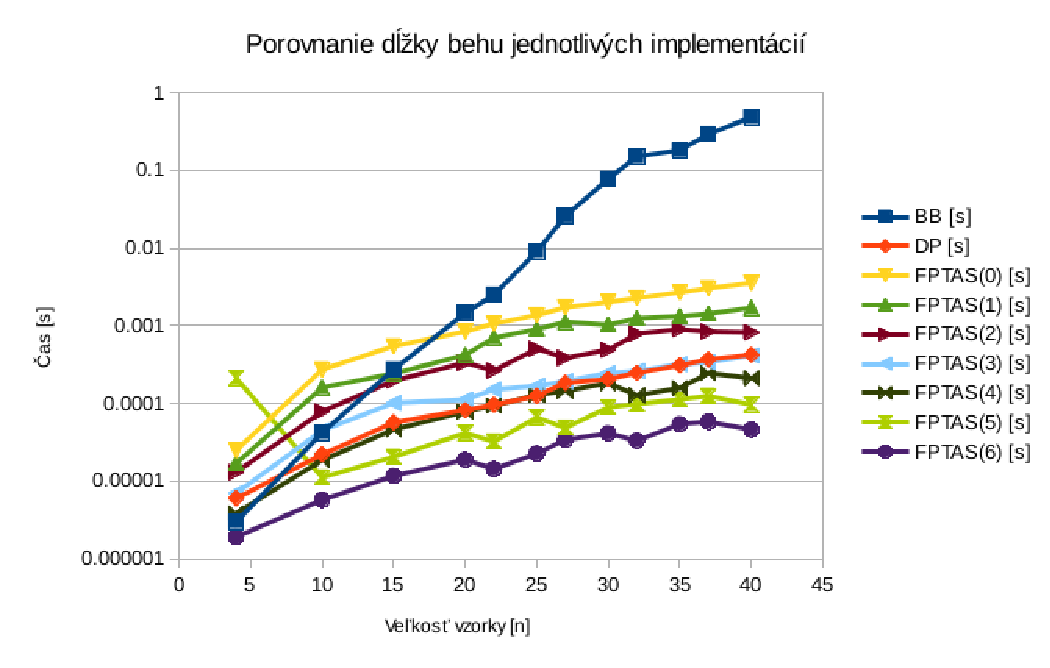
\includegraphics[scale=0.8]{./cas.pdf}
	\caption{Priemerné trvanie jednotlivých implementácií}
	\label{gr:graf1}
\end{figure}

\begin{figure}\centering
	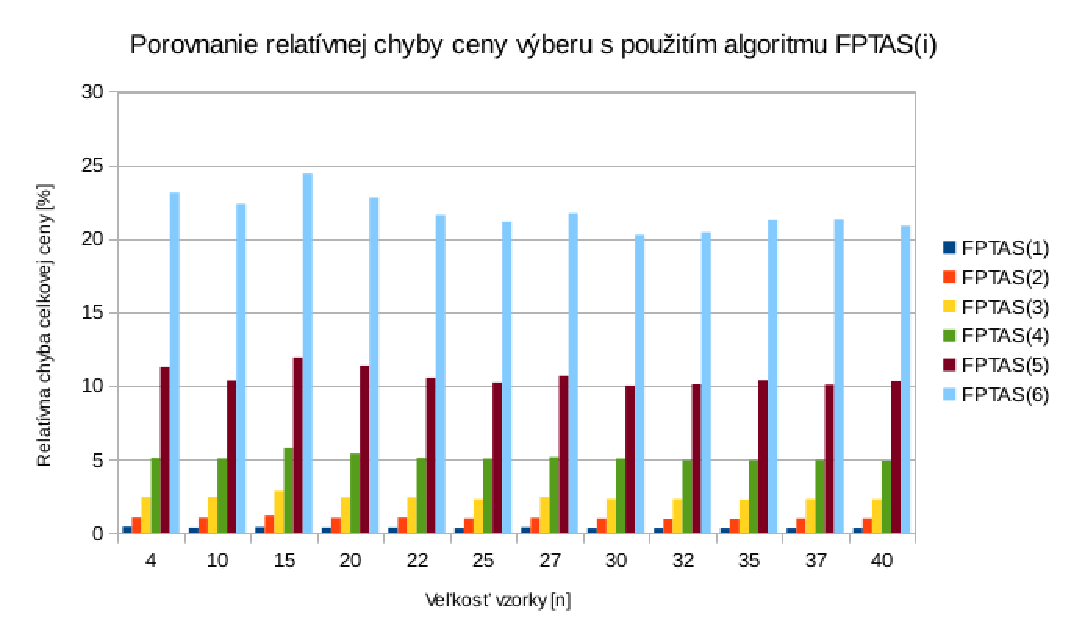
\includegraphics[scale=0.8]{./chyba.pdf}
	\caption{Priemerná relatívna chyba algoritmu FPTAS(i)}
	\label{gr:graf2}
\end{figure}

\begin{figure}\centering
	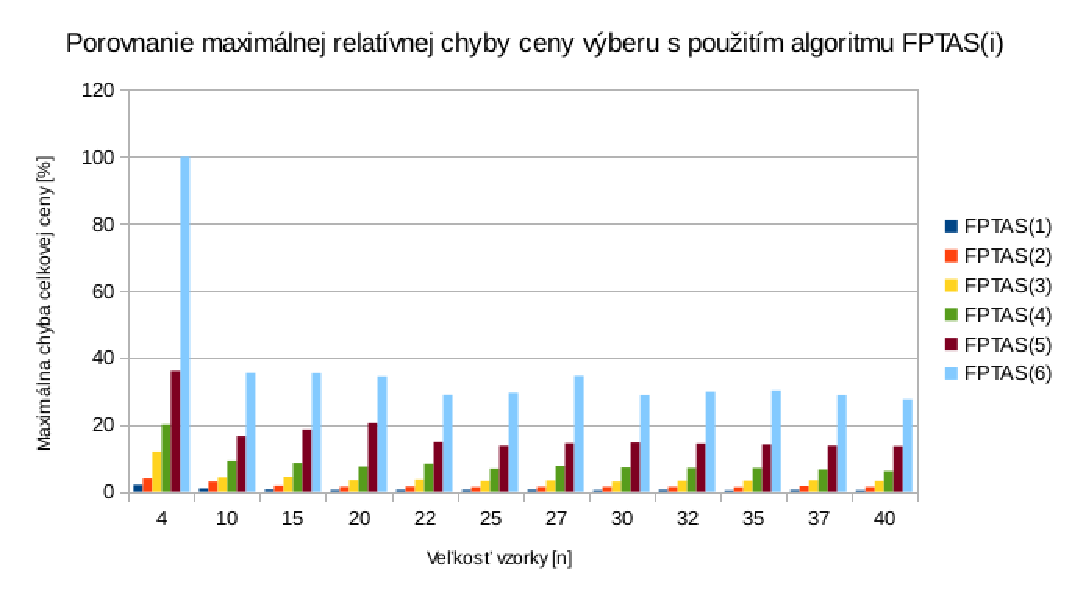
\includegraphics[scale=0.8]{./chyba2.pdf}
	\caption{Maximálna relatívna chyba algoritmu FPTAS(i)}
	\label{gr:graf3}
\end{figure}

\end{document}
